\documentclass[9pt]{beamer}
% \documentclass[9pt,handout]{beamer}
% \documentclass[9pt,draft]{beamer}

\usepackage{amsthm}
\usepackage{amsmath}
\usepackage{amsfonts}
\usepackage{amssymb}

\usepackage[sfdefault, lf, light, semibold]{FiraSans}
% \usepackage[sfdefault]{FiraSans}

\usepackage[]{lucbmath}
\usepackage{bbm}
\usepackage[T1]{fontenc}

\usepackage{minted}

\usetheme[titleformat section=smallcaps,
          titleformat title=smallcaps,
          numbering=none,
          progressbar=foot,
          block=fill]{metropolis}

\definecolor{ared}{rgb}{.647,.129,.149}
\definecolor{white}{HTML}{FAFAFA}
% \setbeamercolor{alerted text}{fg=ared}
\setbeamercolor{progress bar}{fg=ared}


\theoremstyle{definition}
%\renewtheorem{def}{Definition}[section]
\newtheorem{remark}{Remark}
\newtheorem{ex}{Example}
\newtheorem*{theorem?}{Conjecture}
%\renewtheorem{lemma}{Lemma}[section]
\newtheorem{proposition}{Proposition}
\newtheorem{note*}{Note}
% \newtheorem{corollary}{Corollary}
\newtheorem{fct}{Fact}
\newtheorem{qst}{Question}
\newtheorem{claim}{Claim}
\newtheorem{prob}{Problem}

\usepackage{multirow}
\usepackage{array}
\usepackage{booktabs}
\usepackage{pgfplotstable}
\usepackage{colortbl}

\newcommand{\Hilbert}{\mathscr{H}}
\newcommand{\SL}{\operatorname{SL}}
\newcommand{\supp}{\operatorname{supp}}
\newcommand{\R}{\mathbb{R}}
\newcommand{\Z}{\mathbb{Z}}
\newcommand{\A}{\mathbb{A}}

\renewcommand{\S}{S}
\newcommand{\Aut}{\operatorname{Aut}}
\newcommand{\SAut}{\operatorname{SAut}}

\newcommand{\comment}[1]{{\footnotesize \color{black!50}{#1}}}
\newcommand{\SymK}[1]{\mathcal{S}_{#1}}

\setbeamertemplate{itemize items}[default]


\title{Symmetry reduction in semidefinite optimization}

\author{\textbf{Marek Kaluba}} \normalsize
\institute{Karlsruhe Institute for Technology/Heidelberg University}
\date{Będlewo, Applied Topology 2022}
% \normalsize \\[0.05in]\textbf{Piotr W. Nowak} \footnotesize{(IMPAN, Warsaw, Poland)}
% \normalsize \\[0.05in]\textbf{Narutaka Ozawa} \footnotesize{(RIMS, Kyoto, Japan)}}
% \normalsize \\[0.05in]\textbf{Dawid Kielak} \footnotesize{Universitat Bielefeld, Bielefeld, Germany}}

\begin{document}
% \footnotesize
% \firaextralight
\frame{\titlepage}

\begin{frame}[standout]{Outline}
\begin{itemize}
   \item Motivation
   \item Semidefinite programming
  %  \item Computational example
   \item Group Symmetry
   \item Projections, group algebras and beyond
\end{itemize}
\end{frame}


\section{Motivation}

\begin{frame}[standout]
  Given a polynomial $f \in \mathbb{R}[\mathbf{x}]$ is $f$ globally non-negative?

  \pause
  \begin{itemize}
    \item Easy to check refutation (find an $x\in \mathbb{R}^n$ such that $f(x) < 0$).
    \item Does there exist a \textit{witness} for confirmation that is also easy to verify?
  \end{itemize}

\end{frame}

\begin{frame}{Positivity}

  \begin{itemize}
     \item \textbf{analytic}: the value $f(x) \geqslant 0 $ for every $x \in \mathbb{R}^n$
     \item \textbf{algebraic}: $f\in \mathbb{R}[\mathbf{x}]$ admits an algebraic structure which forces it to be positive
  \end{itemize}

  \pause
  \begin{itemize}
    \item $f = ax^2 + bx + c \geqslant 0$ if and only if $a \geqslant 0$ and $b^2 - 4ac \leqslant 0$.
  \pause
    \item We say that $f$ admits a sum of squares (SOS) decomposition when
    \[
    f = \sum_i f_i^2\quad \text{for some } f_i \in \mathbb{R}[\mathbf{x}].
    \]
  \end{itemize}
  \pause
  \begin{example}[Motzkin, 1967]
    $x^4y^2 + x^2y^4 - 3 x^2y^2 + 1 \geqslant 0$ but not SOS.
  \end{example}
\end{frame}

\begin{frame}{Hilbert's 17th problem}

\begin{theorem}[Hilbert, 1888]
  An everywhere non-negative polynomial $p\in \Sigma^2\mathbb{R}[x_1,\ldots, x_n]$ (is a sum of squares) if and only if either
  \begin{itemize}
    \item $n = 1$ (univariate), or
    \item $\operatorname{deg}p = 2$ (quadratic), or
    \item $n = 2$ and $\operatorname{deg}p = 4$ (bivariate quartic).
  \end{itemize}

\end{theorem}
\pause
\begin{theorem}[Artin, 1924]
  An everywhere non-negative polynomial $p$ is a sum of squares of rational functions.
  (i.e. $\exists q\in \mathbb{R}[\mathbf{x}]$ such that  $q^2 p \in \Sigma^2\R[\mathbf{x}]$.
\end{theorem}

\begin{problem}
  How to find such sum of squares (SOS) decomposition?
\end{problem}

\end{frame}

% \begin{frame}

% \begin{itemize}
%   \item $p\in \R[x_1,\ldots, x_d]$ is \textit{positive} iff $p(t) \geqslant 0$ for all $t \in\R^d$ $\Longrightarrow $ \textbf{analytic positivity}.
%   \item $p\in \R[x_1,\ldots, x_d]$ is \textit{positive} iff $p$ is a sum of squares (of rational functions) $\Longrightarrow$ \textbf{algebraic positivity}.
%   \pause
%   \item \textbf{Positivstellensätze} relate one to another.

% \end{itemize}
% \pause
% \begin{problem}
%   How to find such sum of squares (SOS) decomposition?
% \end{problem}
% \end{frame}

\begin{frame}{SOS decompositions}
  \pause
  We can write $f$ as a \textbf{quadratic function of monomials}.
  \begin{example}
  \[
  f = 4x^4 + 4x^3y - 7x^2y^2 - 2xy^3 + 10y^4
  \]
  can be written as
  \[ f =
  \begin{bmatrix}
     x^2, xy, y^2
  \end{bmatrix}
  \begin{bmatrix}
     4         & 2               & -\lambda\\
     2         & -7 + 2\lambda   & -1\\
     -\lambda  & -1              & 10\\
  \end{bmatrix}
  \begin{bmatrix}
   x^2 \\
   xy \\
   y^2 \\
  \end{bmatrix}
  = \mathbf{x}^T P(\lambda) \mathbf{x}
  \]
  \end{example}
  \pause
  $P$ is so called \textbf{Gramm matrix} for $f$.

\end{frame}

\begin{frame}{Quadratic function of monomials}

  \begin{lemma}
  $f$ admits a sum of squares decomposition iff there exists a \textbf{positive semidefinite} Gramm matrix for some (sub)basis $\mathbf{x}$ of $\R[x_1, \ldots x_n]$.
  \end{lemma}
\pause
\begin{example}
For example for $\lambda = 6$ we have
\[
 P(6) = \begin{bmatrix}
   4  &  2 & -6\\
   2  &  5 & -1\\
   -6 & -1 & 10\\
 \end{bmatrix} = Q^T \cdot Q \quad \text{for }
 Q = \begin{bmatrix}
   0 & 2 &  1\\
   2 & 1 & -3
 \end{bmatrix}
\]
Therefore $f$ admits a SOS decomposition
\[f = \left( 2xy + y^2 \right)^2 + \left(2x^2 + xy - 3y^2 \right)^2.\]
\end{example}

\pause
Note: $Q$ is not unique, especially in the rank deficient case; the number of squares equals the rank of $Q$.

\end{frame}

\begin{frame}{Mathematical Programming}
\textbf{Linear programming:}
\begin{itemize}
   \item optimise linear functional
   \item on the set constrained by hyperplanes (polytope)
\end{itemize}
\pause

\textbf{Semi-definite programming}
\begin{itemize}
   \item optimise linear functional
   \item on a polytope intersected with the cone of PSD matrices (spectrahedron)
   \item weak duality, non-unique solutions
   \item even feasibility is a hard problem!
\end{itemize}

\end{frame}

\begin{frame}

  \begin{example}[Textbook formulation]
    \begin{align*}
      \text{maximise:}\quad  & \langle c^T, P \rangle\\
      \text{subject to:}\quad      & P \succcurlyeq 0\\
            & \langle A_i, P \rangle \geqslant b_i, \qquad i = 1,\ldots, m.
    \end{align*}
\end{example}

\pause

\begin{example}

Is $f(x) = 4x^4 + 4x^3y - 7x^2y^2 - 2xy^3 + 10y^4$ always non-negative?
$\Leftarrow$ sum of squares relaxation: Does there exist psd matrix $P$ s.t.
\[f = \mathbf{x}^T P \mathbf{x} (= \langle \mathbf{x} \mathbf{x}^T, P \rangle) ?\]

% \pause
\comment{
  Feasibility problem with
$$
X =
\begin{bmatrix}
  x^2\\
  xy\\
  y^2
\end{bmatrix},
XX^T =
\begin{bmatrix}
  x^4 & x^3y & x^2y^2\\
  \cdot & x^2y^2 & xy^3\\
  \cdot & \cdot & y^4
\end{bmatrix},
A_{x^4} =
\begin{bmatrix}
  1 & 0 & 0\\
  \cdot & 0 & 0\\
  \cdot & \cdot & 0
\end{bmatrix},
A_{x^3y} =
\begin{bmatrix}
  0 & 1 & 0\\
  \cdot & 0 & 0\\
  \cdot & \cdot & 0
\end{bmatrix},\; \text{etc.}
$$
$b = (b_i)$ is the vector of coefficients of $f$.
}

\end{example}
\end{frame}

\begin{frame}{Problem with scaling}
  For $n$-variate polynomial of degree $2d$:
  \[N = {n + d \choose n},\qquad m = {n + 2d \choose n}.\]
  \pause
  \vspace*{-0.1in}
  \begin{itemize}
    \item interior point solvers ($\mathcal{O}(mN^{3.5} + m^2N^{2.5})$)\\
    {\footnotesize\color{black!50}{CSDP, DSDP, Hypatia, MOSEK, SDPA, ...}}
    \item Alternating Direction Method of Multipliers\\
    {\footnotesize\color{black!50}{CDCS, COSMO, SCS, ...}}
    \item Low rank approximation of $P$, (Scaled) dominantly diagonal matrices, Newton conjugate gradient, Primal-dual hybrid gradient...
  \end{itemize}

  \pause
  \begin{exampleblock}{Block-diagonalization}
     Represent $P$ as block diagonal direct sum of psd matrices:
      \begin{enumerate}
        \item Chordal decomposition \comment{(exploit sparsity pattern in $A_i$s)}
        \item Wedderburn(-Artin) decomposition for matrix algebras \\\comment{(group symmetry, general *-algebras, Jordan algebras, ...)}
      \end{enumerate}
  \end{exampleblock}

\end{frame}

\section{Group symmetry}

\begin{frame}{Invariant problems}
\begin{exampleblock}{Optimization problem}
  \begin{align*}
    \text{maximise:}\quad  & \langle c^T, P \rangle\\
    \text{subject to:}\quad      & P \succcurlyeq 0\\
          & \langle A_i, P \rangle \geqslant b_i, \quad i = 1,\ldots, m.
  \end{align*}
\end{exampleblock}

\begin{itemize}
  \item $G$ is a finite group
  \item $G$ acts linearly, orthogonaly on $\mathbb{R}^n$ (space of variables)
  \item $G$ acts linearly, orthogonaly on $\mathbb{R}^m$ (space of constraints)
\end{itemize}

\end{frame}

\begin{frame}{Invariant Solution}
  \begin{exampleblock}{Optimization problem}
    \begin{align*}
      \text{maximise:}\quad  & \langle c^T, P \rangle\\
      \text{subject to:}\quad      & P \succcurlyeq 0\\
            & \langle A_i, P \rangle \geqslant b_i, \quad i = 1,\ldots, m.
    \end{align*}
  \end{exampleblock}

  \begin{alertblock}{When can we find an invariant solution?}
  \[
    \overline{P} = \frac{1}{|G|}\sum_{g\in G} P^g
  \]
  \end{alertblock}

  \pause
  \begin{itemize}
    \item \only<2>{We want to preserve the objective value:
    \[
      \langle c, \overline{P} \rangle =
      \frac{1}{|G|}\sum_g \langle c, P^g\rangle =
      \frac{1}{|G|}\sum_g \langle c^{g^{-1}}, P\rangle =
      \cdots = \langle c, P\rangle
    \]
    holds e.g. when $c$ is invariant under the $G$-action.}
    \only<3>{$\overline{P} \succcurlyeq 0$ follows from the fact that PSD matrices form a cone.}
    \only<4->{We want to preserve the constraint values: $\langle A_i, \overline{P}\rangle = b_i$:
    \[
      \langle A_i, \overline{P}\rangle =
      \frac{1}{|G|}\sum_g\langle A_i, P^g\rangle =
      \left\langle \frac{1}{|G|}\sum_g A_i^{g^{-1}}, P\right\rangle =
      \langle \overline{A_i}, P\rangle
    \]
    which holds when e.g. $b$ - constant on $G$-orbits.
    }

  \end{itemize}

\end{frame}

\begin{frame}{Group symmetry invariance: Example}
    \begin{block}{Robinson form}
        \[
        R(x,y) = x^6 + y^6 - x^4y^2 - y^4x^2 - x^4 - y^4  + 3x^2y^2 - x^2 - y^2 + 1.
        \]

        $R$ is invariant under the following operations \textbf{on monomials}
        \begin{align*}
          \alpha_1 \colon (x, y) & \mapsto (y, x)\\
          \alpha_2 \colon (x, y) & \mapsto (-y, x)
        \end{align*}
      \comment{$\{ \alpha_1, \alpha_2 \}$ generate a set of $8$ symmetries -- the dihedral group $D_4$.}
    \end{block}
      \pause

    \begin{itemize}
      \item the symmetry of monomials leads to the symmetry of constraints,
      \item the symmetry of monomials leads to the symmetry of the psd matrix $P$.
\pause\item In this case: invariant problem = defining polynomial is invariant!
    \end{itemize}
  \end{frame}

  \begin{frame}[standout]{Misleading quote of the day}

    \begin{quote}
      \noindent The \alert{structure of simplifications} that can be derived from group symmetry 
      does \alert{not depend} on the optimization problem.
    \end{quote}

  \end{frame}

  \begin{frame}
    \begin{block}{When a finite $G$ acts linearly on $\mathbb{R}^n$}
      \pause
      \begin{itemize}
        \item a $G$-invariant subspace $V$ is \textbf{irreducible}
        if its only $G$-invariant subspaces are $\{0\}$ and $V$,
        \item the set of the \textbf{types} of irreducible subspaces is finite,
        \item An action-preserving map between subspaces of different types is $0$.
        % \item We say that a projection $p$ is \textbf{semisimple} if $p$ is equivalent to $\oplus_i q$ for a \textbf{single} irreducible projection $q$.
      \end{itemize}
    \end{block}
    \pause

    \begin{lemma}[Schur]
    Suppose that $M, P$ be two linear $G$-maps, $M = m_1 \oplus m_2$ for two irreducible projections $m_i$
    and such that $MPM^{-1} = P$. Then
    \begin{itemize}
      \pause
      \item if $m_1$ and $m_2$ are of \textbf{different types} then
        $P =
        \begin{bmatrix}
  %       \left[\begin{smallmatrix}
        c_1 I_{d_1} & 0 \\
        0     & c_2 I_{d_2}
  %       \end{smallmatrix}\right]
        \end{bmatrix}
        $;
      \pause
      \item if $m_1$ $m_2$ are of the \textbf{same type}, then
        $P =
        \begin{bmatrix}
  %       \left[\begin{smallmatrix}
        c_{11} I_d & c_{12} I_d \\
        c_{21} I_d & c_{22} I_d
  %       \end{smallmatrix}\right]
        \end{bmatrix}
        \cong
        \begin{bmatrix}
  %       \left[\begin{smallmatrix}
        c_{11} & c_{12}\\
        c_{21} & c_{22}
  %       \end{smallmatrix}\right]
        \end{bmatrix}
        \otimes I_d $;
    \end{itemize}
    \end{lemma}

    \pause
    \alert{Miracle:} When $M = M_g$ are given by a linear $G$-action they can be
    \alert{simultaneously} diagonalized to isotypical blocks!

  \end{frame}

  \begin{frame}{Block decomposition from symmetries}
    $P$ is invariant under group symmetries $\iff$ $M_g P M_g^{-1} = P$ for every $g \in G$ $\Longrightarrow$
    $P$ admits a block-diagonal structure.

  \pause

  \begin{center}
  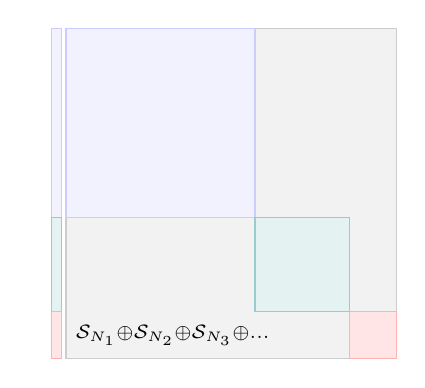
\begin{tikzpicture}[scale=0.6]
  \draw [thin, draw=black!20, fill=black!5] (-0.8,0) (-0.3,7) rectangle (-0.1,0);
  \pause

  \draw [thin, draw=black!20, fill=black!5] (0,0) (7,7) rectangle (0,0);
  \pause
  \draw [thin, draw=blue!20, fill=blue!5] (-0.3,7) rectangle (-0.1,3);
  \draw [thin, draw=teal!40, fill=teal!10] (-0.3,3) rectangle (-0.1,1);
  \draw [thin, draw=red!30, fill=red!10] (-0.3,1) rectangle (-0.1,0);
  \pause
  \draw [thin, draw=blue!20, fill=blue!5] (0,7) rectangle (4,3);
  \draw [thin, draw=teal!40, fill=teal!10] (4,3) rectangle (6,1);
  \draw [thin, draw=red!30, fill=red!10] (6,1) rectangle (7,0);
  \node () at (0,0.5) [anchor=west]
      {${\scriptstyle\SymK{N_1} \oplus \SymK{N_2} \oplus \SymK{N_3} \oplus \ldots}$};

  \pause
  % \begin{scope}[shift={(0,0)}]
  % \draw [thin, draw=black!20, fill=black!5] (0,0) rectangle (7,7);
  % \begin{scope}[shift={(0,3)}, scale=1.333]
  %   \draw [thin, draw=blue!20, fill=blue!5] (0,0) grid (3,3) rectangle (0,0);
  % \end{scope}
  % \draw [thin, draw=teal!40, fill=teal!10] (6,1) grid (4,3) rectangle (6,1);
  % \draw [thin, draw=red!30, fill=red!10] (7,0) grid (6,1) rectangle (7,0);
  % \node () at (0,1) [anchor=west, text width=4cm] {
  %   $\scriptstyle
  %   \left(\mathbb{M}_{m_1}\otimes\SymK{d_1}\right) \oplus
  %   \left(\mathbb{M}_{m_2}\otimes\SymK{d_2}\right) \oplus
  %   \left(\mathbb{M}_{m_3}\otimes\SymK{d_3}\right) \oplus
  %   \ldots$};

  % \begin{scope}[shift={(0,7)}]
  %   \node () at (.66,-.66) [anchor=center] {${\scriptscriptstyle d_1\times d_1}$};
  % \end{scope}

  % \begin{scope}[shift={(4,3)}]
  %   \node () at (.5,-.5) [anchor=center] {${\scriptscriptstyle d_2 \times d_2}$};
  % \end{scope}

  % \begin{scope}[shift={(6,1)}]
  %   \node () at (.5,-.5) [anchor=center] {$\scriptscriptstyle d_3 \times d_3$};
  % \end{scope}


  % \end{scope}

  % \pause


  % \draw [->] (7.3, 3.5) -- (8.7, 3.5);
  % \node () at (8.3, 3.8) [anchor=center, text width=1.3cm] {\tiny by Schur};

  % \begin{scope}[shift={(9,2.5)}, scale=0.25]
  % % \draw [thin, draw=black!20, fill=black!5] (0,0) rectangle (7,7);
  % \begin{scope}[shift={(0,3)}, scale=1.333]
  %   \draw [thin, draw=blue!20, fill=blue!5] (0,0) grid (3,3) rectangle (0,0);
  % \end{scope}
  % % \draw [thin, draw=blue!20, fill=blue!5] (4,3) grid (0,7) rectangle (4,3);
  % \draw [thin, draw=teal!40, fill=teal!10] (6,1) grid (4,3) rectangle (6,1);
  % \draw [thin, draw=red!30, fill=red!10] (7,0) grid (6,1) rectangle (7,0);
  % \node () at (-0.5,-1.5) [anchor=west] {\scriptsize{$\SymK{m_1} \oplus \SymK{m_2} \oplus \SymK{m_3} \oplus \ldots$}};
  % \end{scope}

  % \draw [thin, draw=black!20, fill=black!5] (0,0) grid (7,7) rectangle (0,0);

  \end{tikzpicture}
  \end{center}

  \uncover<6->{\comment{These projections live in the group *-algebra in a basis-free form!}}

  \end{frame}

  \begin{frame}[fragile]{Example: {\texttt{SymbolicWedderburn.jl}}}
  \small
  \begin{minted}{julia}
    using PermutationGroups, DynamicPolynomials
    using SymbolicWedderburn
    G = PermGroup([perm"(1,2)", perm"(1,2,3,4)"]) # Sym(4)
    @polyvar x[1:4];  basis = monomials(x, 0:2) # 15 monomials
    symmetry_adapted_basis(Rational{Int}, G, VariablePermutation(), basis,
        semisimple=true)
  \end{minted}
  \normalsize
  \textbf{Isotypical}/\textbf{semisimple} blocks when acting on \mintinline{julia}|basis|:
  {\scriptsize
  \[
    B_1 = \begin{bmatrix}
            1\\
            x_1 + x_2 + x_3 + x_4\\
            x_{1}x_{2} + x_{1}x_{3} + x_{1}x_{4} + x_{2}x_{3} + x_{2}x_{4} + x_{3}x_{4}\\
            x_{1}^{2} + x_{2}^{2} + x_{3}^{2} + x_{4}^{2}
          \end{bmatrix}
    \qquad
    B_2 = \begin{bmatrix}
          x_{1} - x_{4}\\
          x_{2} - x_{4}\\
          x_{3} - x_{4}\\
          x_{2}^{2} - x_{4}^{2}\\
          x_{3}^{2} - x_{4}^{2}\\
          x_{1}^{2} - x_{4}^{2}\\
          x_{1}x_{2} - x_{3}x_{4}\\
          x_{1}x_{3} - x_{2}x_{4}\\
          x_{1}x_{4} - x_{2}x_{3}\\
          \end{bmatrix}
    \qquad
    B_3 = \begin{bmatrix}
          x_{1}x_{2} - x_{1}x_{4} - x_{2}x_{3} + x_{3}x_{4}\\
          x_{1}x_{3} - x_{1}x_{4} - x_{2}x_{3} + x_{2}x_{4}
          \end{bmatrix}
  \]
  }

  \comment{We went from $15\times 15$-psd constrain to sizes $(4\times 4, 9\times 9, 2\times 2)$.}
    %\[V \cong (V_1' \oplus V_1') \oplus V_2' \oplus V_3', \qquad m_1 = 2, \quad m_2 = m_3 = 1.\]
  \end{frame}

\begin{frame}{Group algebra and projections}
  \begin{definition}{Group algebra $\R[G]$}
    \begin{itemize}
      \item elements of $\R[G]$ are (finitely supported) functions $a\colon G \to \R$, usually written as $a = \sum_g a_g g$
      \pause
      \item multiplication is convolution: if $a = \sum_{g} a_g g$ and $b = \sum_{g} b_g g$ then \[ab = \sum_g \sum_h a_{gh^{-1}}b_h g\]
      \pause e.g. $(1e-2g)(g + 3g^{-1} h^2) = 1g - 2g^{2} + 3g^{-1}h^2 - 6h^{2}$.
    \end{itemize}
    \end{definition}

    \pause
    \begin{block}{Fact:}
    Projections onto isotypical subspaces live in $\mathbb{R}[G]$ in a matrix-free form.
    \end{block}
    \vspace*{-0.2in}
    \pause
    \[
    B_3 = \begin{bmatrix}
      x_{1}x_{2} - x_{1}x_{4} - x_{2}x_{3} + x_{3}x_{4}\\
      x_{1}x_{3} - x_{1}x_{4} - x_{2}x_{3} + x_{2}x_{4}
      \end{bmatrix}\\
    % \intertext{corresponds to}
    \longleftrightarrow
    \tiny
    p_3 = \frac{1}{12}\begin{pmatrix}
      2() - (2,4,3) -(2,3,4)  + 2(1,2)(3,4)  - \\
      (1,3,2)  - (1,4,2)  - (1,4,3)  + (1,3)(2,4)  - \\
      (1,2,3)  + 2(1,4)(2,3)  - (1,2,4)  - (1,3,4)
    \end{pmatrix}
    \]
\end{frame}

\begin{frame}

\begin{center}
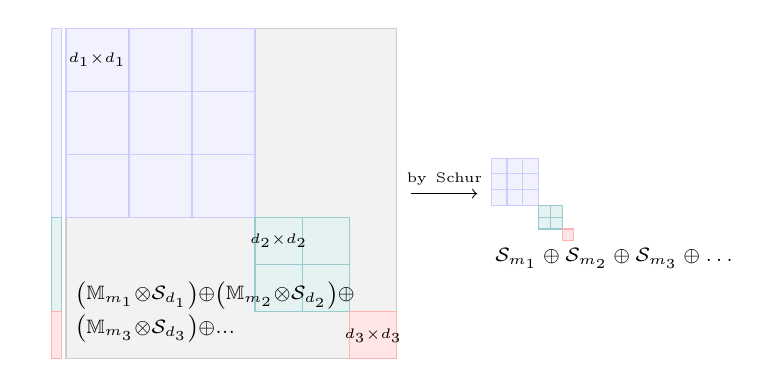
\begin{tikzpicture}[scale=0.6]
\draw [thin, draw=black!20, fill=black!5] (-0.8,0) (-0.3,7) rectangle (-0.1,0);

\draw [thin, draw=black!20, fill=black!5] (0,0) (7,7) rectangle (0,0);

\draw [thin, draw=blue!20, fill=blue!5] (-0.3,7) rectangle (-0.1,3);
\draw [thin, draw=teal!40, fill=teal!10] (-0.3,3) rectangle (-0.1,1);
\draw [thin, draw=red!30, fill=red!10] (-0.3,1) rectangle (-0.1,0);

\draw [thin, draw=blue!20, fill=blue!5] (0,7) rectangle (4,3);
\draw [thin, draw=teal!40, fill=teal!10] (4,3) rectangle (6,1);
\draw [thin, draw=red!30, fill=red!10] (6,1) rectangle (7,0);
\node () at (0,0.5) [anchor=west]
    {${\scriptstyle\SymK{N_1} \oplus \SymK{N_2} \oplus \SymK{N_3} \oplus \ldots}$};

\pause
\begin{scope}[shift={(0,0)}]
\draw [thin, draw=black!20, fill=black!5] (0,0) rectangle (7,7);
\begin{scope}[shift={(0,3)}, scale=1.333]
  \draw [thin, draw=blue!20, fill=blue!5] (0,0) grid (3,3) rectangle (0,0);
\end{scope}
\draw [thin, draw=teal!40, fill=teal!10] (6,1) grid (4,3) rectangle (6,1);
\draw [thin, draw=red!30, fill=red!10] (7,0) grid (6,1) rectangle (7,0);
\node () at (0,1) [anchor=west, text width=4cm] {
  $\scriptstyle
  \left(\mathbb{M}_{m_1}\otimes\SymK{d_1}\right) \oplus
  \left(\mathbb{M}_{m_2}\otimes\SymK{d_2}\right) \oplus
  \left(\mathbb{M}_{m_3}\otimes\SymK{d_3}\right) \oplus
  \ldots$};

\begin{scope}[shift={(0,7)}]
  \node () at (.66,-.66) [anchor=center] {${\scriptscriptstyle d_1\times d_1}$};
\end{scope}

\begin{scope}[shift={(4,3)}]
  \node () at (.5,-.5) [anchor=center] {${\scriptscriptstyle d_2 \times d_2}$};
\end{scope}

\begin{scope}[shift={(6,1)}]
  \node () at (.5,-.5) [anchor=center] {$\scriptscriptstyle d_3 \times d_3$};
\end{scope}


\end{scope}

\pause

\draw [->] (7.3, 3.5) -- (8.7, 3.5);
\node () at (8.3, 3.8) [anchor=center, text width=1.3cm] {\tiny by Schur};

\begin{scope}[shift={(9,2.5)}, scale=0.25]
% \draw [thin, draw=black!20, fill=black!5] (0,0) rectangle (7,7);
\begin{scope}[shift={(0,3)}, scale=1.333]
  \draw [thin, draw=blue!20, fill=blue!5] (0,0) grid (3,3) rectangle (0,0);
\end{scope}
% \draw [thin, draw=blue!20, fill=blue!5] (4,3) grid (0,7) rectangle (4,3);
\draw [thin, draw=teal!40, fill=teal!10] (6,1) grid (4,3) rectangle (6,1);
\draw [thin, draw=red!30, fill=red!10] (7,0) grid (6,1) rectangle (7,0);
\node () at (-0.5,-1.5) [anchor=west] {\scriptsize{$\SymK{m_1} \oplus \SymK{m_2} \oplus \SymK{m_3} \oplus \ldots$}};
\end{scope}

% \draw [thin, draw=black!20, fill=black!5] (0,0) grid (7,7) rectangle (0,0);

\end{tikzpicture}
\end{center}

\uncover<4->{
\[
  B_3' = \frac{1}{2}\begin{pmatrix}
    \scriptstyle
    x_{1}x_{2} - x_{1}x_{4} - x_{2}x_{3} + x_{3}x_{4} + \\
    \scriptstyle
    x_{1}x_{3} - x_{1}x_{4} - x_{2}x_{3} + x_{2}x_{4}
    \end{pmatrix}
  % \intertext{corresponds to}
  \longleftrightarrow
  q_3\cdot p_3\quad \text{where } q_3 = \frac{1}{2}\left(() + (3,4)\right)
\]
}

\uncover<5->{
\begin{block}{Open problem}
  Given an isotypical projection $p \in \R[G]$ how to find
  a projection $q \in \R[G]$ so that $p(q) = 1$?
\end{block}
}

\end{frame}

  \begin{frame}[fragile]{Example: {\texttt{SymbolicWedderburn.jl}}}
  \vspace*{0.2in}
  \scriptsize

  \begin{minted}{julia}
    # [ ... ]
    symmetry_adapted_basis(Rational{Int}, G, VariablePermutation(), basis
      [, semisimple=false])
  \end{minted}
  \normalsize
  \textbf{Simple} blocks when acting on \mintinline{julia}|basis|:
  \tiny
  \[
    B_1' = \begin{bmatrix}
            1\\
            x_1 + x_2 + x_3 + x_4\\
            x_{1}x_{2} + x_{1}x_{3} + x_{1}x_{4} + x_{2}x_{3} + x_{2}x_{4} + x_{3}x_{4}\\
            x_{1}^{2} + x_{2}^{2} + x_{3}^{2} + x_{4}^{2}
          \end{bmatrix}
    \qquad
    B_2' = \begin{bmatrix}
          \frac{1}{3}(3x_{1} - x_{2} - x_{3} - x_{4})\\
          \frac{1}{3}(3x_{1}^{2} - x_{2}^{2} - x_{3}^{2} - x_{4}^{2})\\
          x_{1}x_{2} + x_{1}x_{3} + x_{1}x_{4} - x_{2}x_{3} - x_{2}x_{4} - x_{3}x_{4}
          \end{bmatrix}
  \]
  \[
    B_3' = \begin{bmatrix}
          \frac{1}{2}(2x_{1}x_{2} - x_{1}x_{3} - x_{1}x_{4} - x_{2}x_{3} - x_{2}x_{4} + 2x_{3}x_{4})
          \end{bmatrix}
  \]

  \comment{Reduction: $15\times 15 \to (4\times 4, 9\times 9, 2\times 2) \to (4\times 4, 3\times 3, 1\times 1)$-psd constraints.}\\[0.1in]

  \end{frame}

  \begin{frame}{Large scale example}

  Optimization problem from geometric group theory\footnote{Kaluba, M., Nowak, P.W. \& Ozawa, N. $\operatorname{Aut}(F_5)$ has property (T). \textit{Math. Ann}. \textbf{375}, 1169–1191 (2019). \url{https://doi.org/10.1007/s00208-019-01874-9}}:
  \begin{block}{Estimate the spectral gap of the group Laplacian for $\operatorname{Aut}(F_5)$}
     If $\Delta^2 - \lambda \Delta \geqslant 0$ then $(0, \lambda)$ is not in the spectrum.
  \end{block}
  \pause
    \begin{itemize}
      \item relax $\Delta^2 - \lambda \Delta \geqslant 0$ as sum of squares problem:
      \pause
      \item psd-constraint of size $4\,641\times 4\,641$, $~1.1\cdot 10^7$ constraints
      \item symmetry group: $S_2 \wr S_5$ ($3840$ elements)
      \item After symmetrization:
        \begin{itemize}
          \item $29$-blocks (largest: $58\times 58$) ($13\,232$ variables in total)
          \item $7\,230$ constraints
        \end{itemize}
      \item Solvable in 20 minutes to $\varepsilon \sim 10^{-12} $!
    \end{itemize}

  \end{frame}

  \begin{frame}
  \begin{center}
  \vfill
  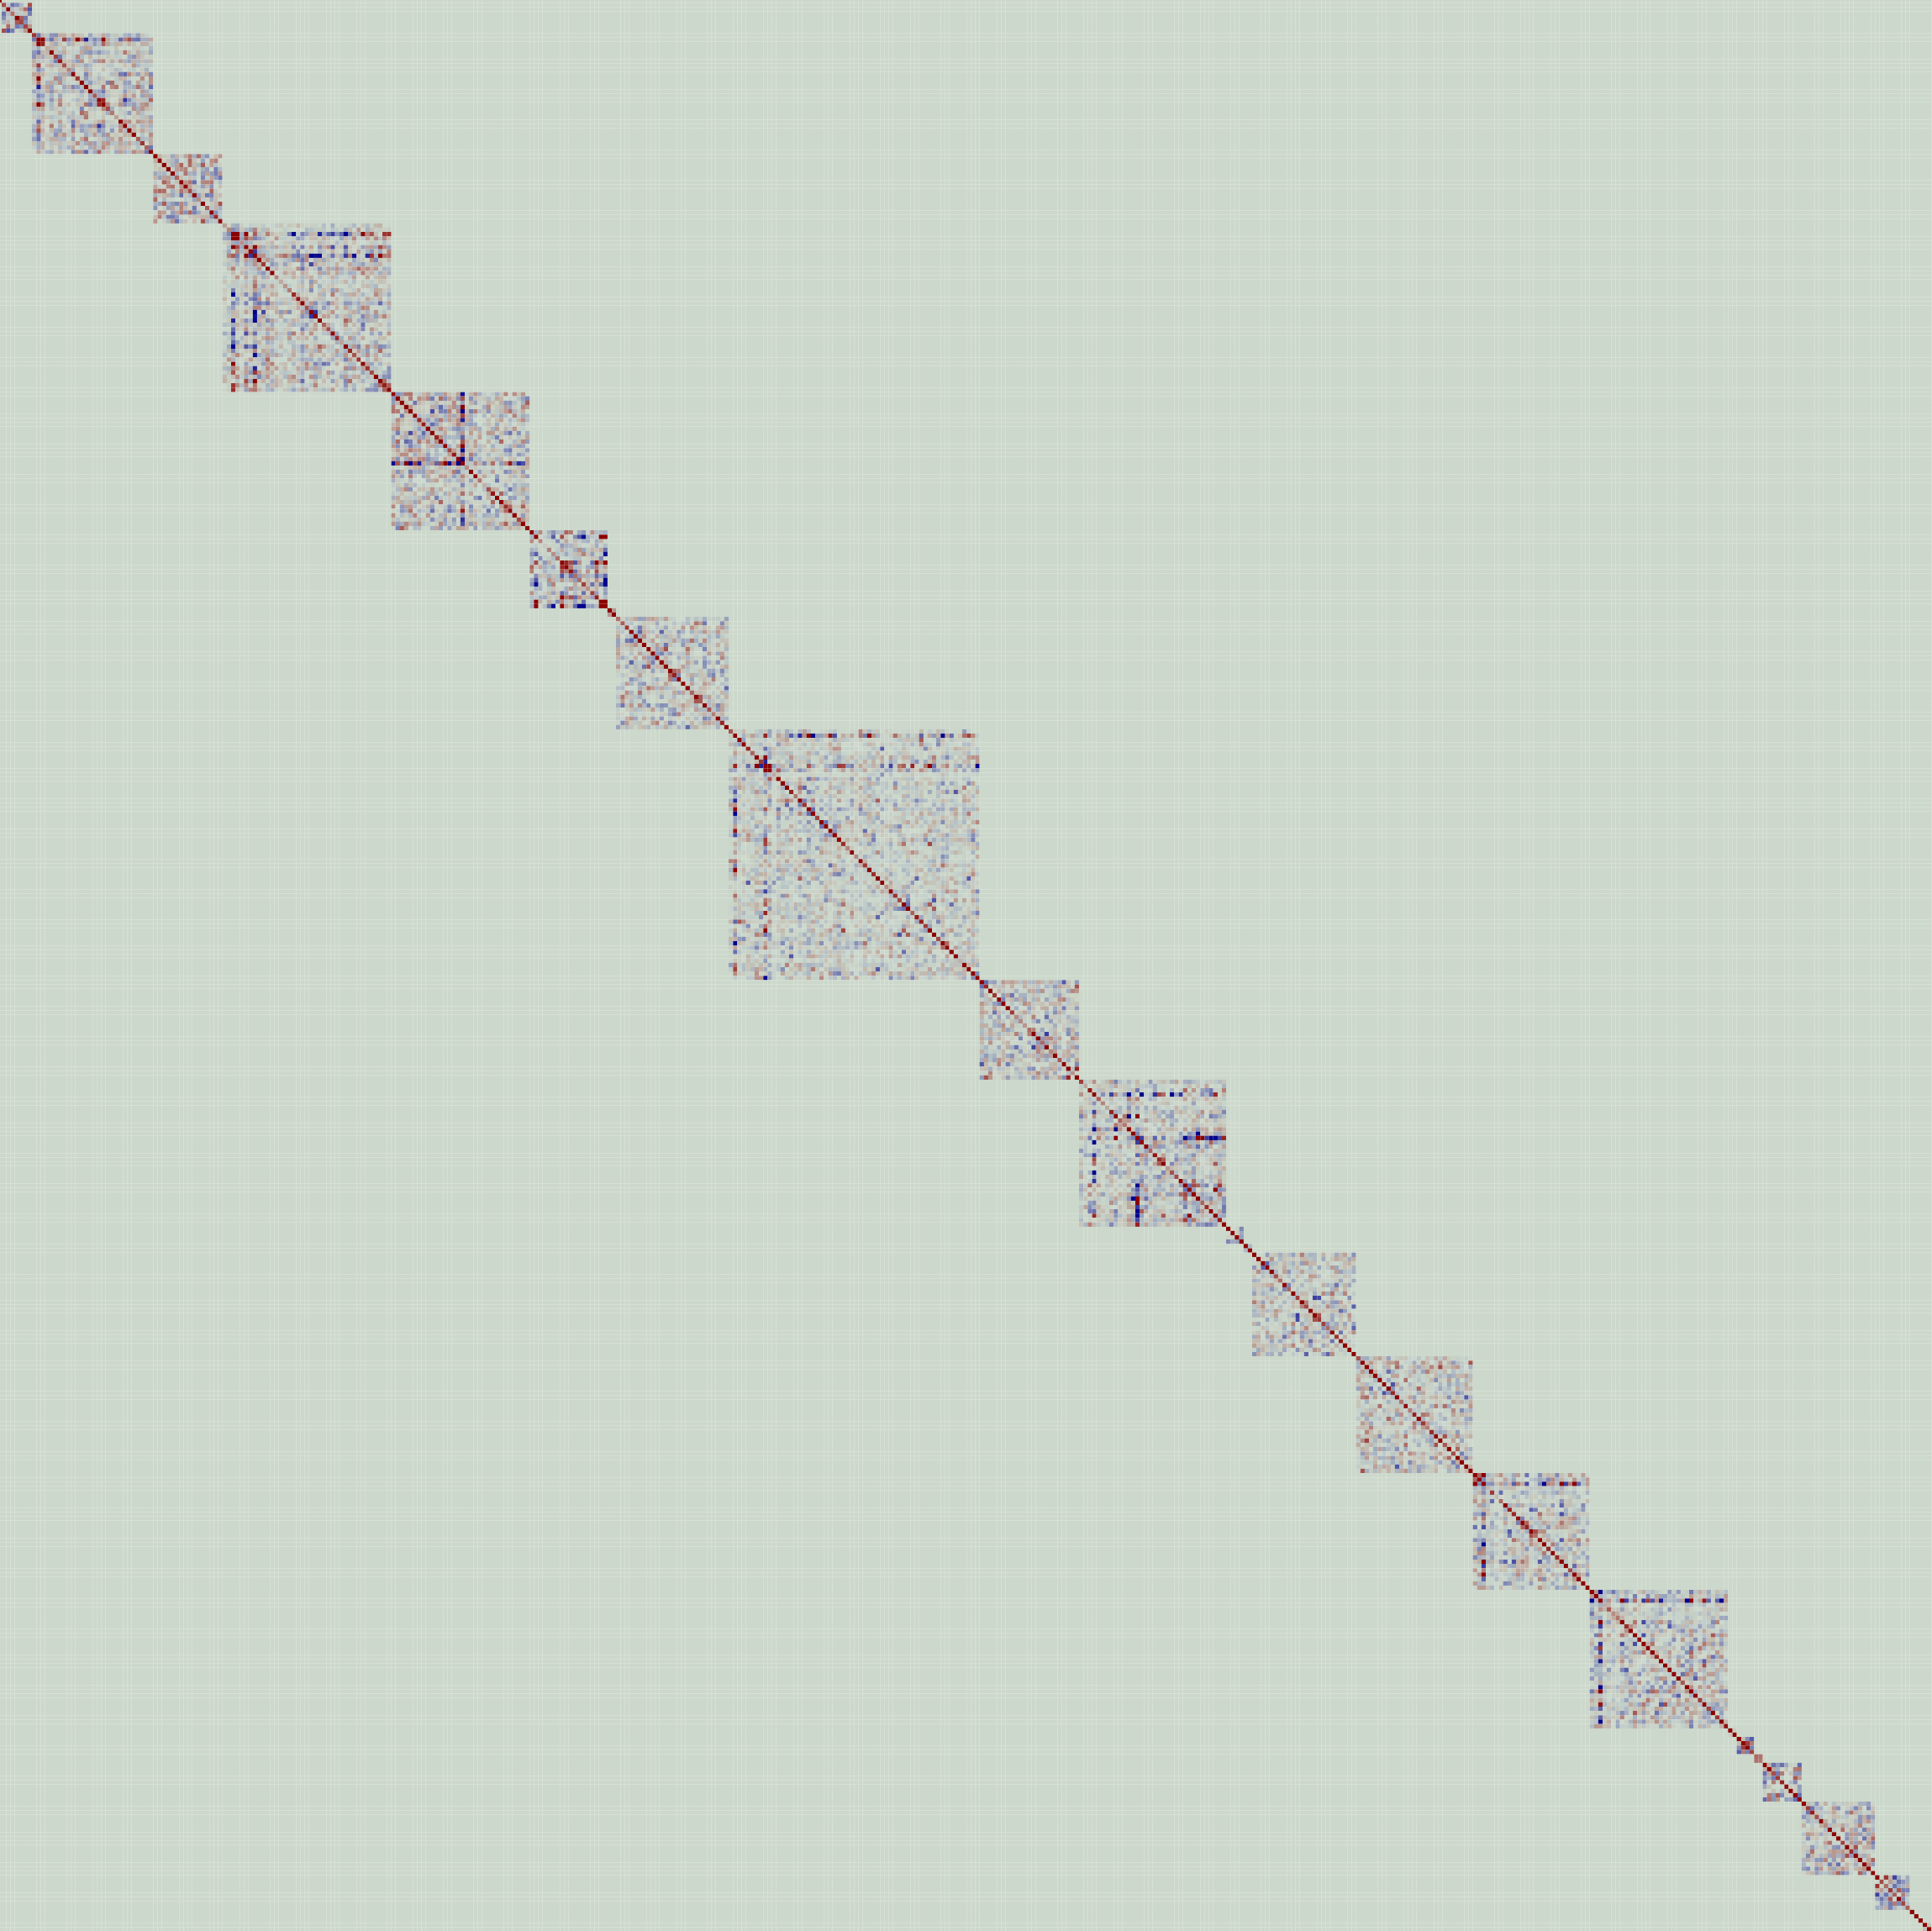
\includegraphics[height=\textheight]{AutF5_blocks.png}
  \vfill
  \end{center}
  \end{frame}

  \begin{frame}
  \centering
  \begin{tikzpicture}[scale=0.9]
  \draw [thin, draw=black!20, fill=blue!5] (0,0) grid (10.18,-10.18) rectangle (0,0);
  \node at (6.5, -9.5) {Original psd constraint ($4\, 641 \times 4\, 641$)};
  \node (ssdp) at (.5,-.5) {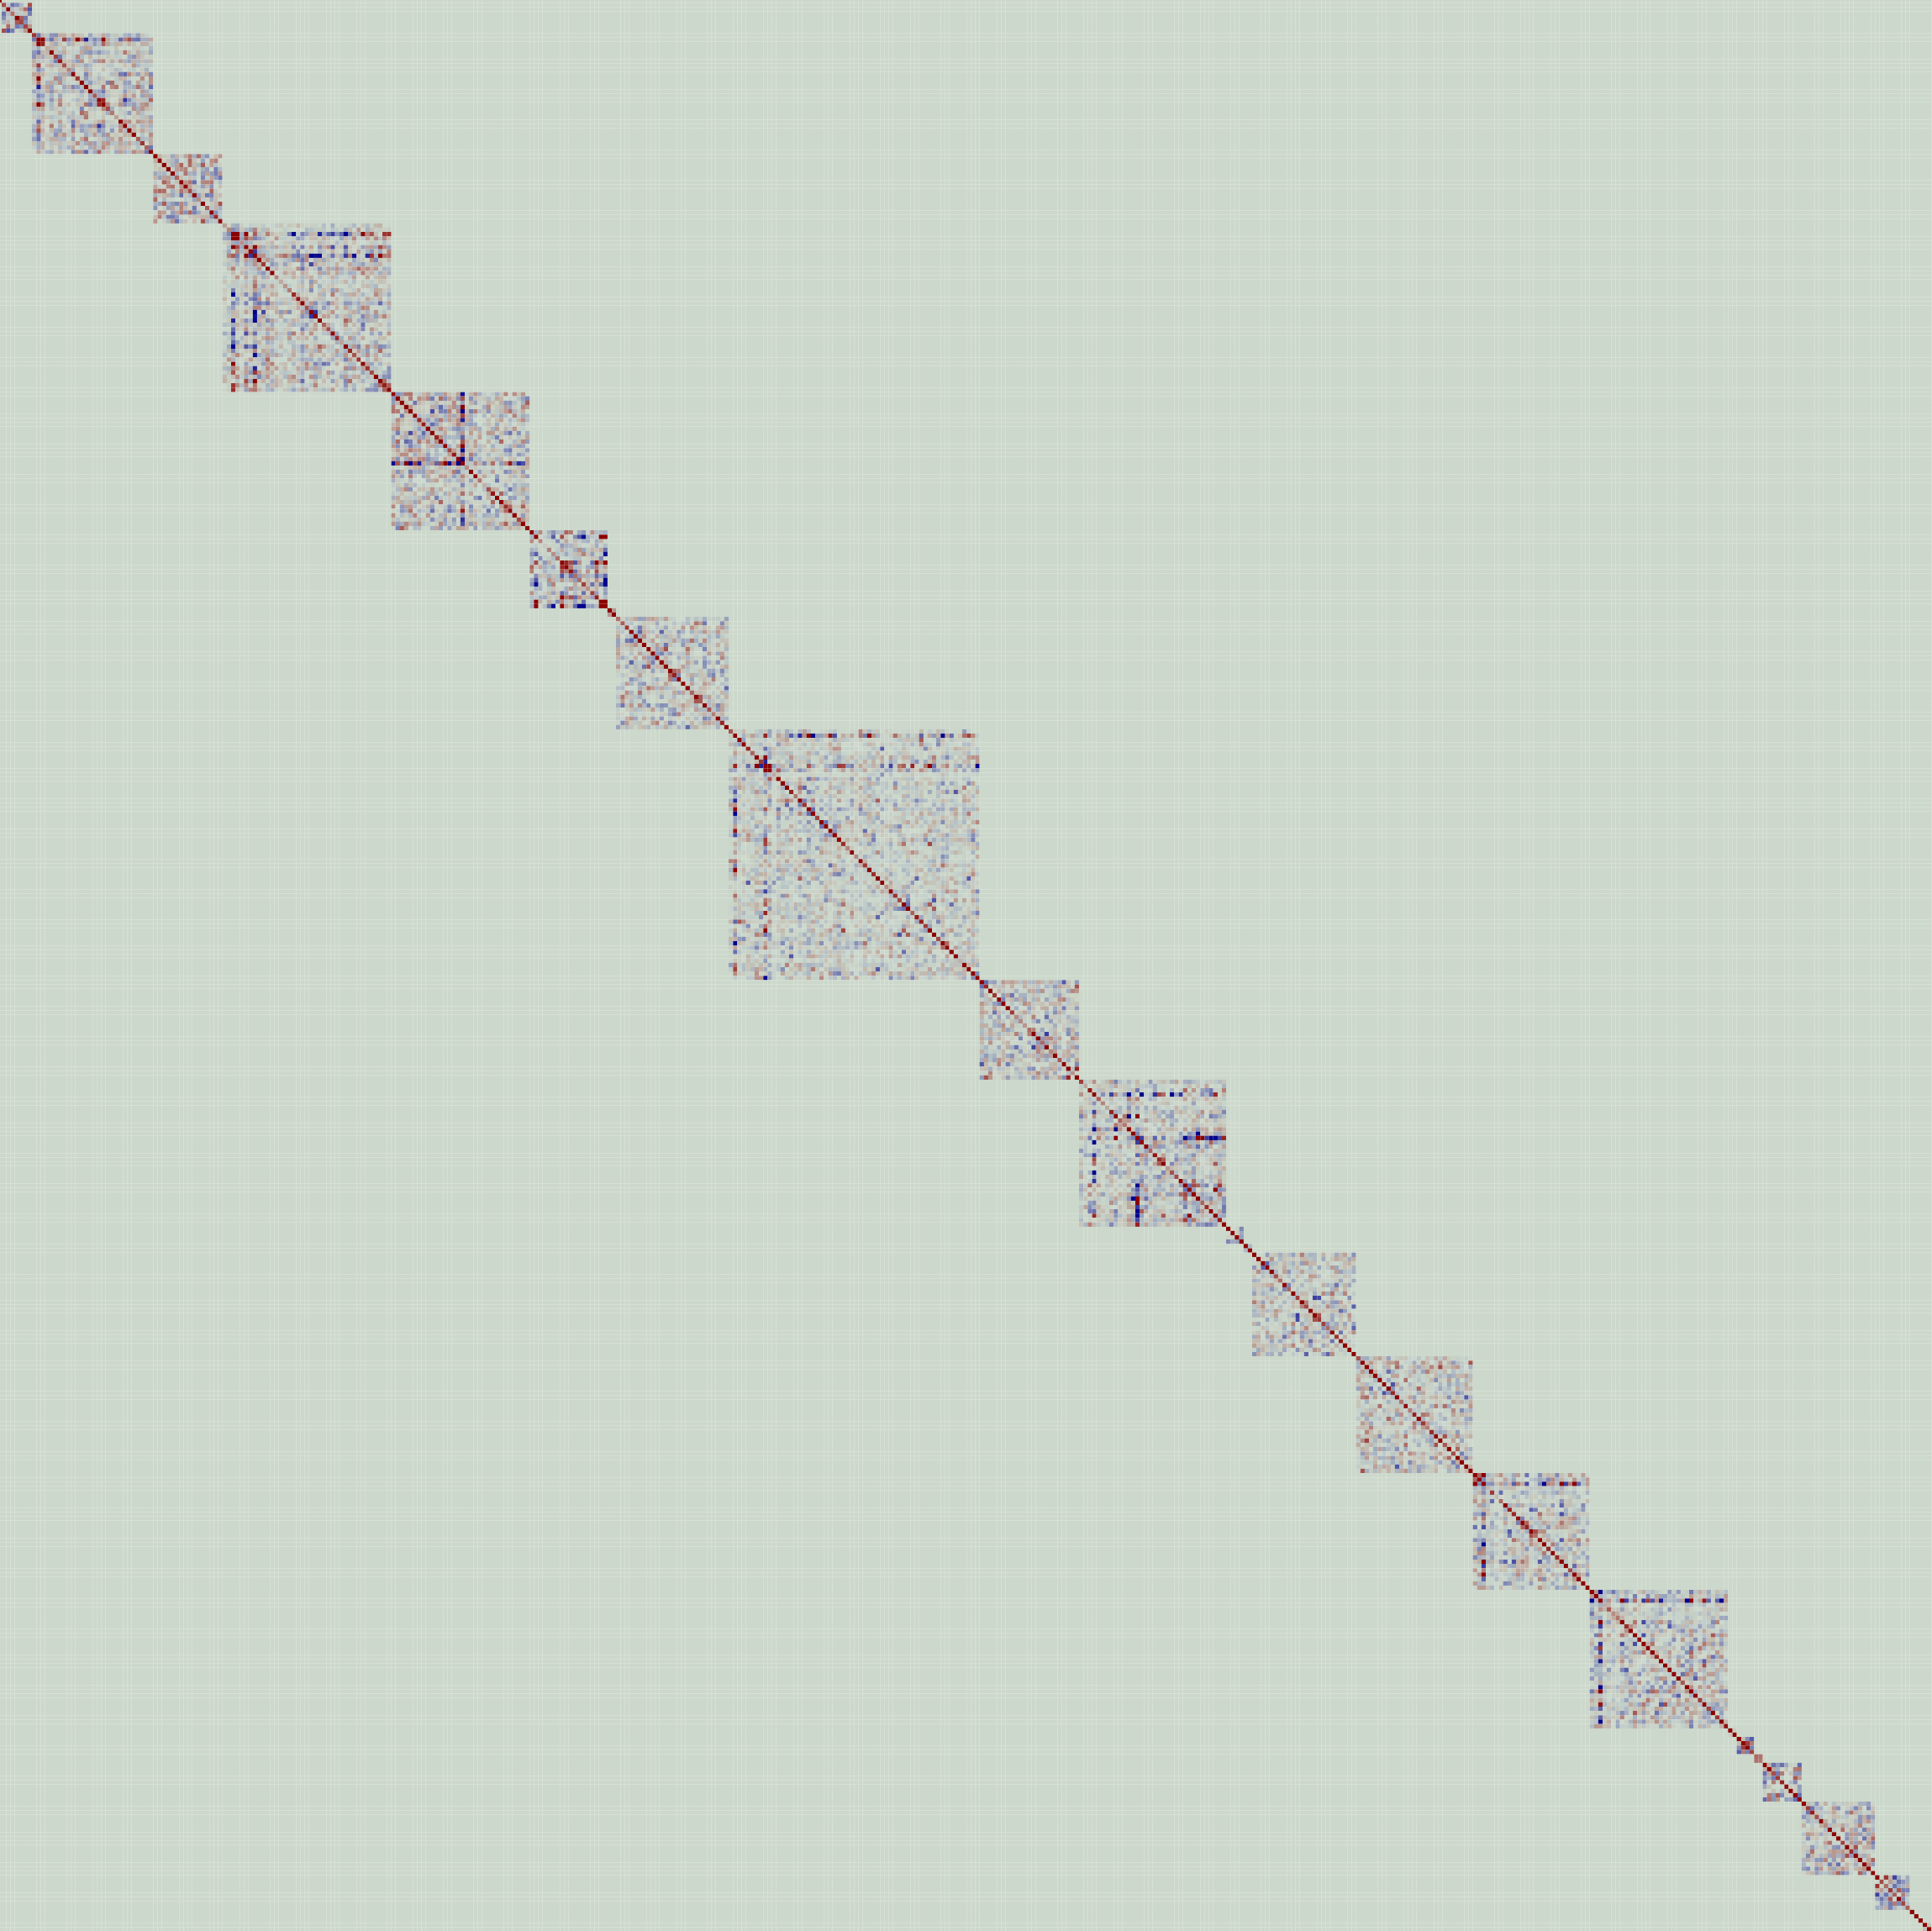
\includegraphics[width=0.9cm]{AutF5_blocks.png}};
  \node (label) at (4.5,-.5) {diagonalized psd ($\subset 448\times 448$)};
  \draw [->] (label.west) -- (ssdp.east);
  \end{tikzpicture}


  \end{frame}


\end{document}



% \begin{frame}[standout]
%    And now for something completely different:
%    \\
%    it's example time!
% \end{frame}

% \end{document}


\begin{frame}{NC positivity: $*$-algebras}

\pause
To state Positivstellensatz in the NC-setting we need \textbf{algebras with involution} (i.e. $*$-algebras).

\pause
\begin{example}
  \begin{itemize}[<+->]
    \item $\R[x_1,\ldots, x_d]$, $p \mapsto p$
    \item $\mathbb{C}[x_1,\ldots, x_d]$, $p \mapsto \overline{p}$ (conjugation on coefficients)
    \item $\mathbb{C}[z, z^{-1}]$ (Laurent polynomials) $\sum_{k=-N}^{N} a_k z^{k} \mapsto \sum_{k=-N}^{N} \overline{a_k} z^{-k}$
    \item $\mathbb{C}[\mathbb{Z}] \cong \mathbb{C}[z, z^{-1}]$ (the complex group algebra of integers)
    \item $\R\langle x_1, \ldots, x_d \rangle$, $p \mapsto p$ (free polynomial algebra, i.e. variables don't commute!)
    \item $\R[G]$, the involution $*\colon \R[G] \to \R[G]$ induced by $g \mapsto g^{-1}$ (and trivial on $\R$) gives $\R[G]$ the structure of $*$-algebra, e.g. \[(1e-2g + 3g^{-1} h^2)^* = 1e - 2g^{-1} + 3h^{-2}g.\]
  \end{itemize}
\end{example}
\end{frame}

\begin{frame}{NC sums of squares}
    \begin{definition}
    If $\A $ is a $*$-algebra, then the cone of sum of squares (quadratic module) is defined as
    \[\Sigma^2\A  = \left\{\sum_{i=1}^n \xi_i^* \xi_i \colon \quad \xi_i\in \A ,\quad n\in \mathbb{N} \right\}.\]
    \pause Note: each $p\in \Sigma^2\A $ is fixed by $*$.
  \end{definition}
  \pause
  \begin{multline*}
    \Delta = |\S|e - \sum_{g\in \S} g = \frac{1}{2}\left(2|\S|e - \sum_{g\in \S} g^* + g\right) = \frac{1}{2} \sum_{g\in \S} \left( 2e - g^* - g \right) =
    \\= \frac{1}{2} \sum_{g\in \S}(1-g)^*(1-g)
  \end{multline*}
\end{frame}

\begin{frame}{NC positivity}

  \begin{example}[Free polynomial algebra]
    An element $a=\sum_g a_g g \in \R\langle x_1, \ldots, x_d\rangle$
    is \textbf{positive} if $a = a^*$ and for all $n\in \mathbb{N}$ and for every choice of matrices $A = (A_1, \ldots, A_d)$, each $A_i\in M_n(\R)$,
    \[\varphi_A(a) = \sum_g a_g \varphi_A(g) \succcurlyeq 0,\]
    where $\varphi_A$ replaces $x_i$ by $A_i$ for all $i$.
  \end{example}

  \pause
  \begin{itemize}
    \item This corresponds directly to evaluation of polynomials: the only representations of polynomial rings are
    \[\varphi_t (p) = p(t) \quad \text{ for $t$ in $\R^d$}.\]
    \item \pause If there are non-trivial relations between $x_i$s (or the $*$-involution on $\A $ is not trivial) we need the matrices $A_1, \ldots, A_n$ to be compatible: this leads to \textbf{$*$-algebra representations}.
  \end{itemize}
\end{frame}


\begin{frame}{NC positivity}
  \begin{definition}
  Let $\mathcal{H}$ be a (real) Hilbert space.
  \begin{itemize}[<+->]
  \item
    A $*$-representation of $\A $ on $\mathcal{H}$ is an algebra homomorphism $\varphi\colon \A  \to \operatorname{End}(\mathcal{H})$, so that $\varphi(1)v = v$ and $\varphi(a^*)$ is adjoint to $\varphi(a)$, i.e.
    \[\langle\varphi(a)v,w \rangle = \langle v, \varphi(a^*)w \rangle\]
    for all $v,w\in \mathcal{H}$ and $a\in \A $.
%   \item We write $\varphi(a) \geqslant 0$ when $\langle\varphi(a)v,v \rangle \geqslant 0$ for all $v\in \mathcal{H}$.
  \item For a family $\mathcal{F}$ of $*$-representations define
  \[\A (\mathcal{F})_{\geqslant} = \{a \in \A \colon\quad a^* = a,\quad \varphi(a)\succcurlyeq 0 \text{ for all } \varphi\in \mathcal{F}\}\]
  \end{itemize}
  \end{definition}

%   \textbf{Positivstellensätze} are interplays between $\A (\mathcal{F})_{\geqslant}$ and $\Sigma^2 \A $.

\end{frame}

\begin{frame}{NC-Positivstellensatz}
  \begin{theorem}[Schmüdgen, Henkel, ...]
    Let $\A $ be the commutative $*$-algebra $\mathbb{C}[x_1, \ldots, x_d]$, or free $*$-algebra $\mathbb{C}\langle x_1, \ldots, x_d \rangle$.
    If $a \in \A$ s.t. $a = a^*$ then the following are equivalent:
    \begin{enumerate}
      \item $a\in \A (\mathcal{F})_{\geqslant}$ where $\mathcal{F}$ is the family of all $*$-representations of $\A $
      \item $a \in \Sigma^2 \A$
    \end{enumerate}
  \end{theorem}

  \pause
  Many different other cases known (Weyl algebras, quantum groups, enveloping algebras, in some cases group algebras ...).

  \pause

  \begin{theorem}[Abstract Positivstellensatz]
    Assume that $u$ is an interior point of $\Sigma^2 \A$.
    If $a \in \A$ s.t. $a = a^*$ then the following are equivalent
    \begin{enumerate}
      \item $a \in \A(\mathcal{F})_{\geqslant}$ where $\mathcal{F}$ is the family of all $*$-representations of $\A$
      \item $a + \varepsilon u \in \Sigma^2 \A$ for all $\varepsilon>0$, where $u$ is an interior point of $\Sigma^2 \A$.
    \end{enumerate}
  \end{theorem}

\end{frame}

\begin{frame}[standout]
  Example application
  \begin{itemize}
    \item $\blacktriangleright\;$ group $G$ property (T) is hard analytic property;
    \item $\blacktriangleright\;$ (T) reduces to the positivity of a specific element in group algebra: \[\Delta^2 - \lambda\Delta \in \R[G]\]
    \item $\blacktriangleright\;$ Schmüdgen gives sums of squares approach
    \begin{flushright}
    \pause\normalsize (as long as we know some interior points $u$)
    \end{flushright}
  \end{itemize}

\end{frame}


\begin{frame}{NC-Positivstellensatz for $\R[G]$}
    \begin{itemize}
      \pause
      \item $\xi \geqslant 0 \iff \pi(\xi) \succcurlyeq 0$ in every $*$-representation of $\R [G]$
      \pause
      \item $\Sigma^2\R[G] = \left\{\sum_i \xi_i^* \xi_i\colon \xi\in \R[G]\right\}$% = \left\{\sum_{g,h} P_{g,h}g^{-1}h \colon P\succcurlyeq 0, P\in \mathbb{M}_G\right\}$

    \end{itemize}

   \pause
  \begin{theorem}[Positivstellensatz]
    Assume that $u$ is an interior point of $\Sigma^2 \R [G]$.
    For any $\xi \in \R [G]$ s.t. $\xi^* = \xi$
    \[\xi \geqslant 0 \iff \xi + \varepsilon u \in \Sigma^2 \R [G] \text{ for all $\varepsilon>0$ (and some $\lambda>0$)?}\]
   \end{theorem}
    \pause
    \begin{example}[Property (T)]
%        \begin{itemize}
%            \item
        $1e$ is an interior point of $\Sigma^2 \R [G]$, i.e. \[\text{Is}\quad \Delta^2 - \lambda\Delta +\varepsilon e \in \Sigma^2\R [G] \quad\text{for all $\varepsilon$?}\] \pause This of no use for us: SOS decompositions $\Delta^2 - \lambda\Delta + \varepsilon e = \sum\xi_i^*\xi_i$ may be very diffrent for different $\varepsilon$.

%        \end{itemize}
   \end{example}
\end{frame}

\begin{frame}{NC-Positivstellensatz}
    Let $I[G] = \left\{\sum_g a_g g \colon \sum_g a_g = 0\right\}$ be the augmentation ideal.\pause
    \begin{proposition}
        $\Delta$ is an interior point of $\Sigma^2 I[G] = I[G] \cap \Sigma^2\R[G]$\pause, i.e. \\for any $\xi \in I[G]$ s.t. $\xi^* = \xi$
        \[ \xi \geqslant 0 \iff \xi + \varepsilon \Delta \in \Sigma^2 I[G]\quad \text{for all $\varepsilon > 0$.}\]
    \end{proposition}
\pause
    \begin{example}
       If we can show that $\Delta^2 - \lambda \Delta + \varepsilon_0 \Delta = \sum \xi_i^* \xi_i$ for a single fixed $\varepsilon_0$, then \[\Delta^2 - (\lambda-\varepsilon_0)\Delta + \varepsilon\Delta = \sum\xi_i^* \xi_i + \varepsilon \sum (1-g)^* (1-g) \in \Sigma^2 I[G]\]
       \pause for all $\varepsilon $ simultanuously!
    \end{example}

\end{frame}


\begin{frame}{Action Plan}
   \pause
   \begin{enumerate}[<+->]
      \item Pick $G = \langle \S |\mathcal{R}\rangle$;
      \item Set $\vec{\mathbf{x}} = (e, g_1, g_2, \ldots, g_n), \quad g_i\in B_d(e, \S )$ ($d = 2,3,\ldots$);
      \item Solve the problem (numerically):
        \begin{align*}
           \text{maximize:}  \quad & \lambda\\
           \text{subject to:}\quad & P \succcurlyeq 0, \quad P\in \mathbb{M}_{\vec{\mathbf{x}}}\\
           & \lambda \geq 0\\
           & (\Delta^2 - \lambda\Delta)_t = \left(\vec{\mathbf{x}}^* P\vec{\mathbf{x}}^T\right)_t =
           \sum_{g^{-1}h=t} P_{g,h}, \quad \text{for all $t\in B_{2d}(e,\S )$}\\
        \end{align*}
        \item Compute $\sqrt{P} = Q = [\overrightarrow{q_e}, \ldots, \overrightarrow{q_{g_n}}]$
        \item Finally: $\xi_g = \langle \vec{\mathbf{x}}, \overrightarrow{q_g}\rangle$ and $\Delta^2 - \lambda \Delta = \sum_{g\in \vec{\mathbf{x}}}{\xi_g}^*\xi_g.$

   \end{enumerate}

\end{frame}

% \begin{frame}[standout]
%     \begin{quote}
%    How do we certify that the numerical result is sound?
%    \end{quote}
% \end{frame}

% \begin{frame}{Certifying correctness}
%
%     \begin{lemma}[Netzer\&Thom]
%        Let $r\in I[G] \subset \R [G]$ such that $\supp(r) \subset B_d(e)$. Then
%         \[r + 2^{d-1}\|r\|_1\cdot\Delta \in \Sigma^2 I [G].\]
%     \end{lemma}
%
%     \begin{corollary}
%       If $\Delta^2 - \lambda\Delta = \sum \xi_i^*\xi_i + r$, then
%       \[ \Delta^2 - \left(\lambda- 2^{d-1}\|r\|_1\right)\Delta = \sum \xi_i^*\xi_i + \left(r + 2^{d-1}\|r\|_1\Delta\right) \in \Sigma^2 I[G],\]
%       i.e. $\Delta$ has spectral gap of at least $\lambda - 2^{d-1}\|r\|_1$.
%     \end{corollary}
%
%
% \end{frame}
%
% \begin{frame}{Action Plan 2}
%
%    \begin{enumerate}
%       \item Pick $G = \langle \S |\mathcal{R}\rangle$;
%       \item Set $\vec{\mathbf{x}} = (e, g_1, g_2, \ldots, g_n), \quad g_i\in B_d(e, \S )$ ($d = 2,3,\ldots$);
%       \item Solve the problem (numerically):
%       \begin{align*}
%         \text{maximize:}  \quad & \lambda\\
%         \text{subject to:}\quad & P \succcurlyeq 0, \quad P\in \mathbb{M}_{\vec{\mathbf{x}}}\\
%         & \lambda \geq 0\\
%         & (\Delta^2 - \lambda\Delta)_t = \left(\vec{\mathbf{x}}^* P\vec{\mathbf{x}}^T\right)_t, \quad \text{for all $t\in B_{2d}(e,\S )$}\\
%       \end{align*}
%       \vspace*{-0.3in}
%       \item Compute $Q = [\overrightarrow{q_e}, \ldots, \overrightarrow{q_{g_n}}] \sim \sqrt{P}$
%       \uncover<4->{
%         {
%           \color{red}
%           \[P \to \sqrt{P} \to \sqrt{P}_{\textsl{int}} \to \sqrt{P}_{\textsl{int}}^{aug} \to Q \in \mathbb{M}_{\vec{\mathbf{x}}}(\R IF)\]
%         }
%       }
%       \vspace*{-0.2in}
%       \uncover<2->{
%         \item Setting $\xi_g = \langle \vec{\mathbf{x}}, \overrightarrow{q_g}\rangle$ we have
%         \[\Delta^2 - \lambda \Delta = \sum\xi_g^* \xi_g + r,\quad\text{{
%           \color{red}
%           where $r \in I[G]$ and $\|r\|_1< \varepsilon$.
%           }
%         }\]
%       \vspace{-0.15in}
%       }
%       \uncover<3->{
%         \item Finally $\Delta^2 - (\lambda - 2^{d-1}\varepsilon)\Delta = \sum\xi_j^*\xi_j + \left(r + 2^{d-1}\varepsilon\Delta\right) \geq 0$, hence {
%           \color{red}
%           \[\lambda_1(G, \S ) \geq (\lambda - 2^{d-1}\varepsilon) \quad\text{is certified.}\]
%         }
%       }
%    \end{enumerate}
% \end{frame}

\section{Concrete examples}

\begin{frame}
  \begin{itemize}
    \item $\SL(3,\Z)$, $\SL(4,\Z)$, $\SL(5,\Z)$
    \item $\SAut(F_5)$
  \end{itemize}
  \pause
  But also:
  \begin{itemize}
    \item $\SL(n,\Z)$ ($n\geqslant 3$)
    \item $\SAut(F_n)$ ($n\geqslant 5$).
  \end{itemize}
\end{frame}


\begin{frame}{Further reduction in size}

  \begin{itemize}[<+->]
    \item Find a finite group $K$ which acts on $G$ but keeps $\xi$ invariant $\Longrightarrow$ the optimisation problem has a $K$-invariant solution
    \item The left-regular representation of $G$ inherits the $K$-action (by operator conjugation) $\Longrightarrow$ decompose the representation into simple $K$-matrix algebras via Wedderburn decomposition (correspond to irreducible representations of $K$)
    \item Using minimal projection system for $K$ reduce the size of the optimisation problem

    \item Solve the smaller problem and reconstruct the solution $P$ of the larger one.

    \item (note: if $\xi$ is constant on the orbits of the action on $\mathbb{R}[G]$ $\Longrightarrow$ decompose basis of ${R}[G]$ into orbits of $K$)
  \end{itemize}
\end{frame}

\end{document}
